\chapter{Objetivos}
\label{cap:capitulo2}

En el capítulo \ref{cap:capitulo1}, se ha descrito e introducido el contexto en el que se enmarca este \ac{TFG}. En este segundo capítulo, que a continuación se expone, se procederá a presentar los objetivos específicos que se han establecido para este proyecto.

\section{Descripción del problema}
\label{sec:descripcion_problema}

Como se menciona en el primer capítulo, la conducción autónoma promete ser un avance tecnológico que cambie completamente la manera en la que se concibe la movilidad en nuestra sociedad. Este trabajo de fin de grado tiene como principal objetivo realizar una investigación sobre la utilización de distintas técnicas de \ac{IA}, para la creación de una solución completa para la problemática de la navegación por un carril. Se presentará un comportamiento dotado de la capacidad de seguir un carril, adaptarse al tráfico de este y evitar colisiones en caso de que el tráfico se detenga.

\section{Objetivos}
\label{sec:Objetivos}

\begin{enumerate}
	\item Instalación y configuración del simulador CARLA, ROS 2, logrando además una comunicación entre ambos.
	\item Análisis de la viabilidad de desarrollar aplicaciones de conducción autónoma mediante el uso del simulador foto-realista CARLA y el framework de aplicaciones roboticas ROS 2, utilizando \textit{CARLA to ros bridge} como medio de comunicación.
	\item Creación de un comportamiento sigue carril autónomo basado en aprendizaje por refuerzo.
	\item Desarrollar un comportamiento para, además de navegar por un carril de manera segura, detenerse antes de colisionar con obstáculos de la carretera.
	\item Elaboración de un comportamiento que permita a un vehículo adaptarse a la velocidad del tráfico a la hora de navegarautonomamente  por un carril utilizando aprendizaje por refuerzo.
	\item Análisis de métricas de los algoritmos desarrollados en el \ac{TFG} y realización de una comparativa entre estas métricas.
\end{enumerate} 


\section{Requisitos}
\label{sec:requisitos}

Los requisitos que ha de cumplir este trabajo son los siguientes:
\begin{itemize}
	\item El trabajo ha de realizarse en el simulador foto-realista de conducción autónoma CARLA.
	\item Los sistemas a desarrollar deben ser reactivos, es decir deben ser capaces de reaccionar a su entorno de manera rápida y precisa.
	\item El vehículo debe navegar de manera adecuada, natural y segura.
\end{itemize}

\section{Metodología}
\label{sec:metodologia}

El \ac{TFG} comenzó en octubre de 2022 y finalizó también en octubre de 2023. A lo largo de estos 12 meses se siguieron las siguientes directrices para la realización del mismo:
\begin{itemize}
	\item Reuniones semanales el tutor del \acs{TFG} para establecer micro-objetivos semanales y reales. Gracias a estas reuniones, fue fácil mantener un control del avance del proyecto en cada momento e ir solucionando de manera rápida y efectiva los problemas que surgían.
	\item Realización de un blog\footnote{\url{https://roboticslaburjc.github.io/2022-tfg-juancamilo-carmona/}}. en el que se añadían periódicamente entradas con información sobre el avance del proyecto, además de los problemas enfrentados en cada etapa, a modo de bitácora para documentar todo el proceso de desarrollo.
	\item Se utilizó la plataforma de comunicación Microsoft Teams para realizar las reuniones periódicas con mi tutor del TFG y el correo de la universidad para mantener contacto con él en todo momento, con el fin de resolver problemas que pudieran surgir, notificar avances y solicitar consejos.
	\item Se empleó la plataforma de desarrollo GitHub para alojar todo el código desarrollado en el \ac{TFG} \footnote{\url{https://github.com/RoboticsLabURJC/2022-tfg-juancamilo-carmona}}.
	\item En el desarrollo de este \ac{TFG}, se adoptó la metodología Scrum como sistema de trabajo. A lo largo del desarrollo de este trabajo, se establecieron diferentes sprints, cada uno de ellos con una duración determinada, durante los cuales se plantearon mini objetivos específicos a alcanzar. Esta estructura no solo permitió una organización y planificación eficiente del trabajo, sino que también ofreció la flexibilidad necesaria para adaptarse a cambios y nuevos requerimientos que surgieron a lo largo del desarrollo del \ac{TFG}.
	
\begin{figure}[h]
	\centering
	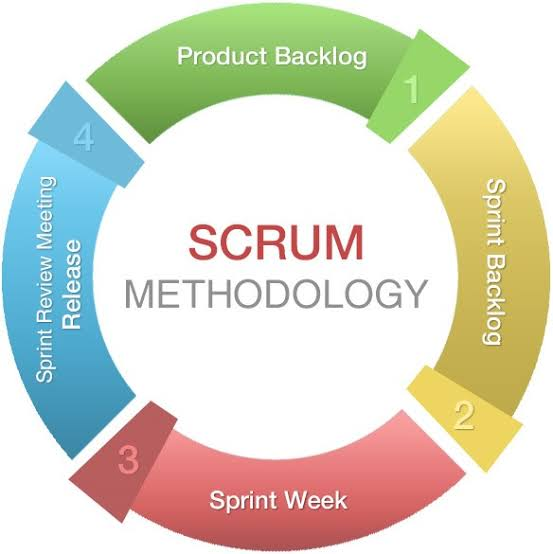
\includegraphics[width=0.5\linewidth]{imagenes/cap2/scrum.jpg}
	\caption{Ilustración de la metodología scrum}
	\label{fig:Ilustración de la metodología scrum}
\end{figure}
\end{itemize}

\section{Plan de trabajo}
\label{sec:plantrabajo}

Durante los 12 meses en los que se ha desarrollado este proyecto, se ha seguido un plan de trabajo con la siguiente estructura:
\begin{enumerate}
	\item Etapa de configuración: Esta etapa consistió básicamente en preparar todo el entorno para la realización del \ac{TFG}. Aquí se instalaron todos los drivers, software y aplicaciones necesarias para empezar a trabajar.
	\item Comienzo del \ac{TFG}: Una vez el entorno de trabajo estaba listo, se empezó a desarrollar todo el código.
	\begin{itemize}
		\item En primer lugar, se inició con el desarrollo de un teleoperador para un vehículo.
		\item En segunda instancia, una vez el teleoperador estaba terminado, se continuó con los algoritmos de seguimiento de carril con percepción basada visión artificial tradicional y un algoritmo con percepción basada en una red neuronal.
		\item Una vez finalizado el desarrollo de los algoritmos de percepción, la siguiente etapa consistió en analizar las métricas de todos ellos y compararlas para llegar a una conclusión sobre la mejor solución para la problemática.
		\item El siguiente paso, fue programar un sigue carril basado en aprendizaje por refuerzo.
		\item Una vez terminado el comportamiento sigue carril, se procedió a añadir un comportamiento el cual permitiera no chocarse al encontrar obstáculos en la carretera.
		\item Finalmente se trabajó en una solución más completa de conducción autónoma que navegara por un carril correctamente, deteniéndose en caso de encontrar un vehículo u obstáculo detenido y adaptándose a la velocidad del tráfico sin colisionar ni ni detener la marcha en caso de que este existiera.
	\end{itemize}
	\item Para finalizar, se procedió a la redacción de la memoria del \ac{TFG}.
\end{enumerate}

